\section{Results}

The following section presents the measured data and the calculated linear expansion coefficients for the three metals.

\begin{figure}[h]
    \centering
    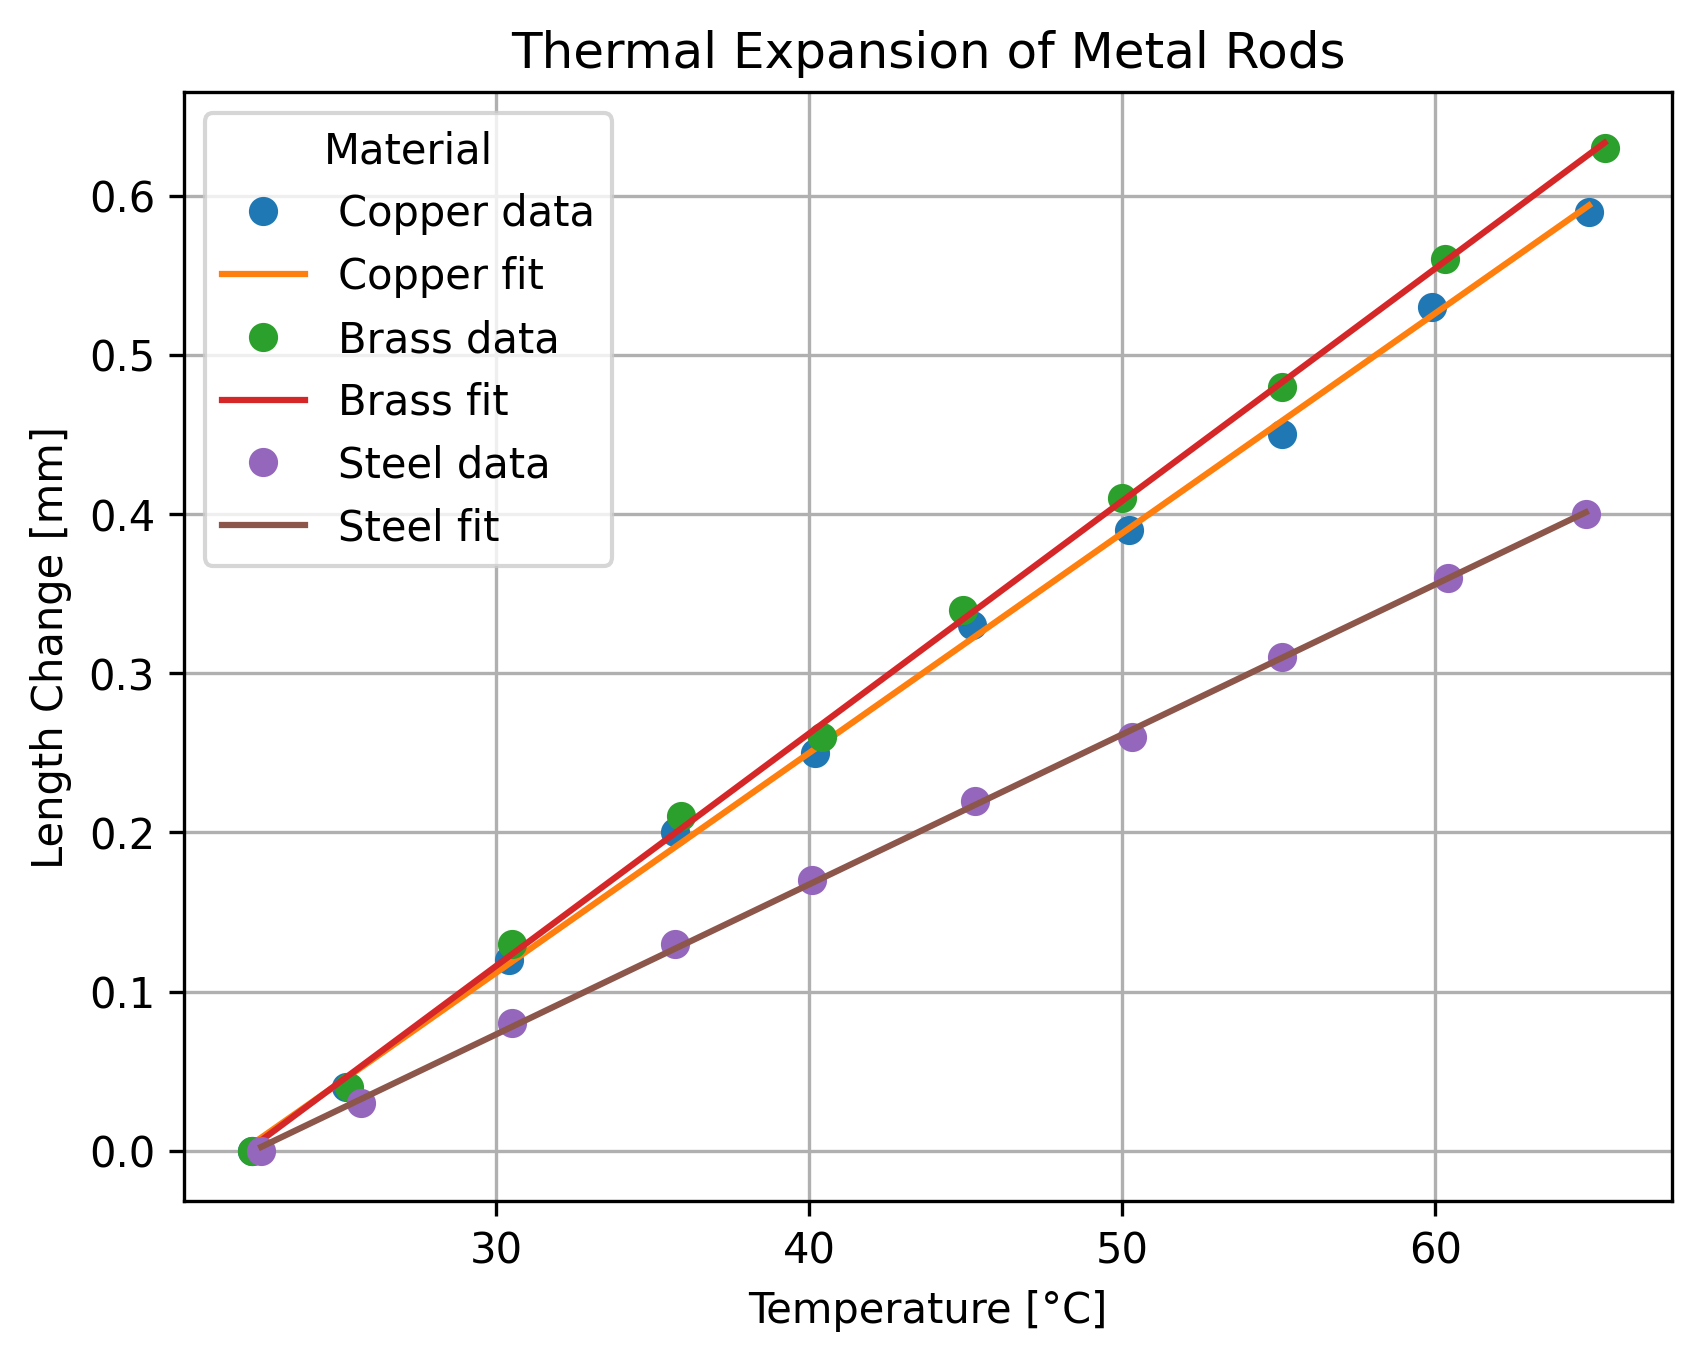
\includegraphics[width=1\textwidth]{figures/expansion_plot.png}
    \caption{Thermal expansion of metal rods.}
    \label{fig:expansion_plot}
\end{figure}

\subsection*{Determined Coefficients}

The coefficients $a$ and the linear expansion coefficient $\alpha$ were calculated using a linear fit of the measured length change $\Delta L$ as a function of temperature $T$ for each metal:

\begin{equation}
    \Delta L = a \, T + b
\end{equation}

Here, $a$ [mm/°C] is the slope of the fitted line, and $b$ is the intercept. The linear expansion coefficient $\alpha$ [1/°C] was then calculated by dividing the slope $a$ by the initial rod length $L_0$:

\begin{equation}
    \alpha = \frac{a}{L_0}
\end{equation}

\begin{table}[H]
\centering
\begin{tabular}{l c c}
\toprule
Metal & $a$ [mm/°C] & $\alpha$ [1/°C] \\
\midrule
Copper & 0.013813 & $1.791 \cdot 10^{-5}$ \\
Brass  & 0.014608 & $1.894 \cdot 10^{-5}$ \\
Steel  & 0.009425 & $1.219 \cdot 10^{-5}$ \\
\bottomrule
\end{tabular}
\caption{Determined linear expansion coefficients.}
\end{table}

\subsection*{Measured Length Changes}

\begin{figure}[H]
    \centering
    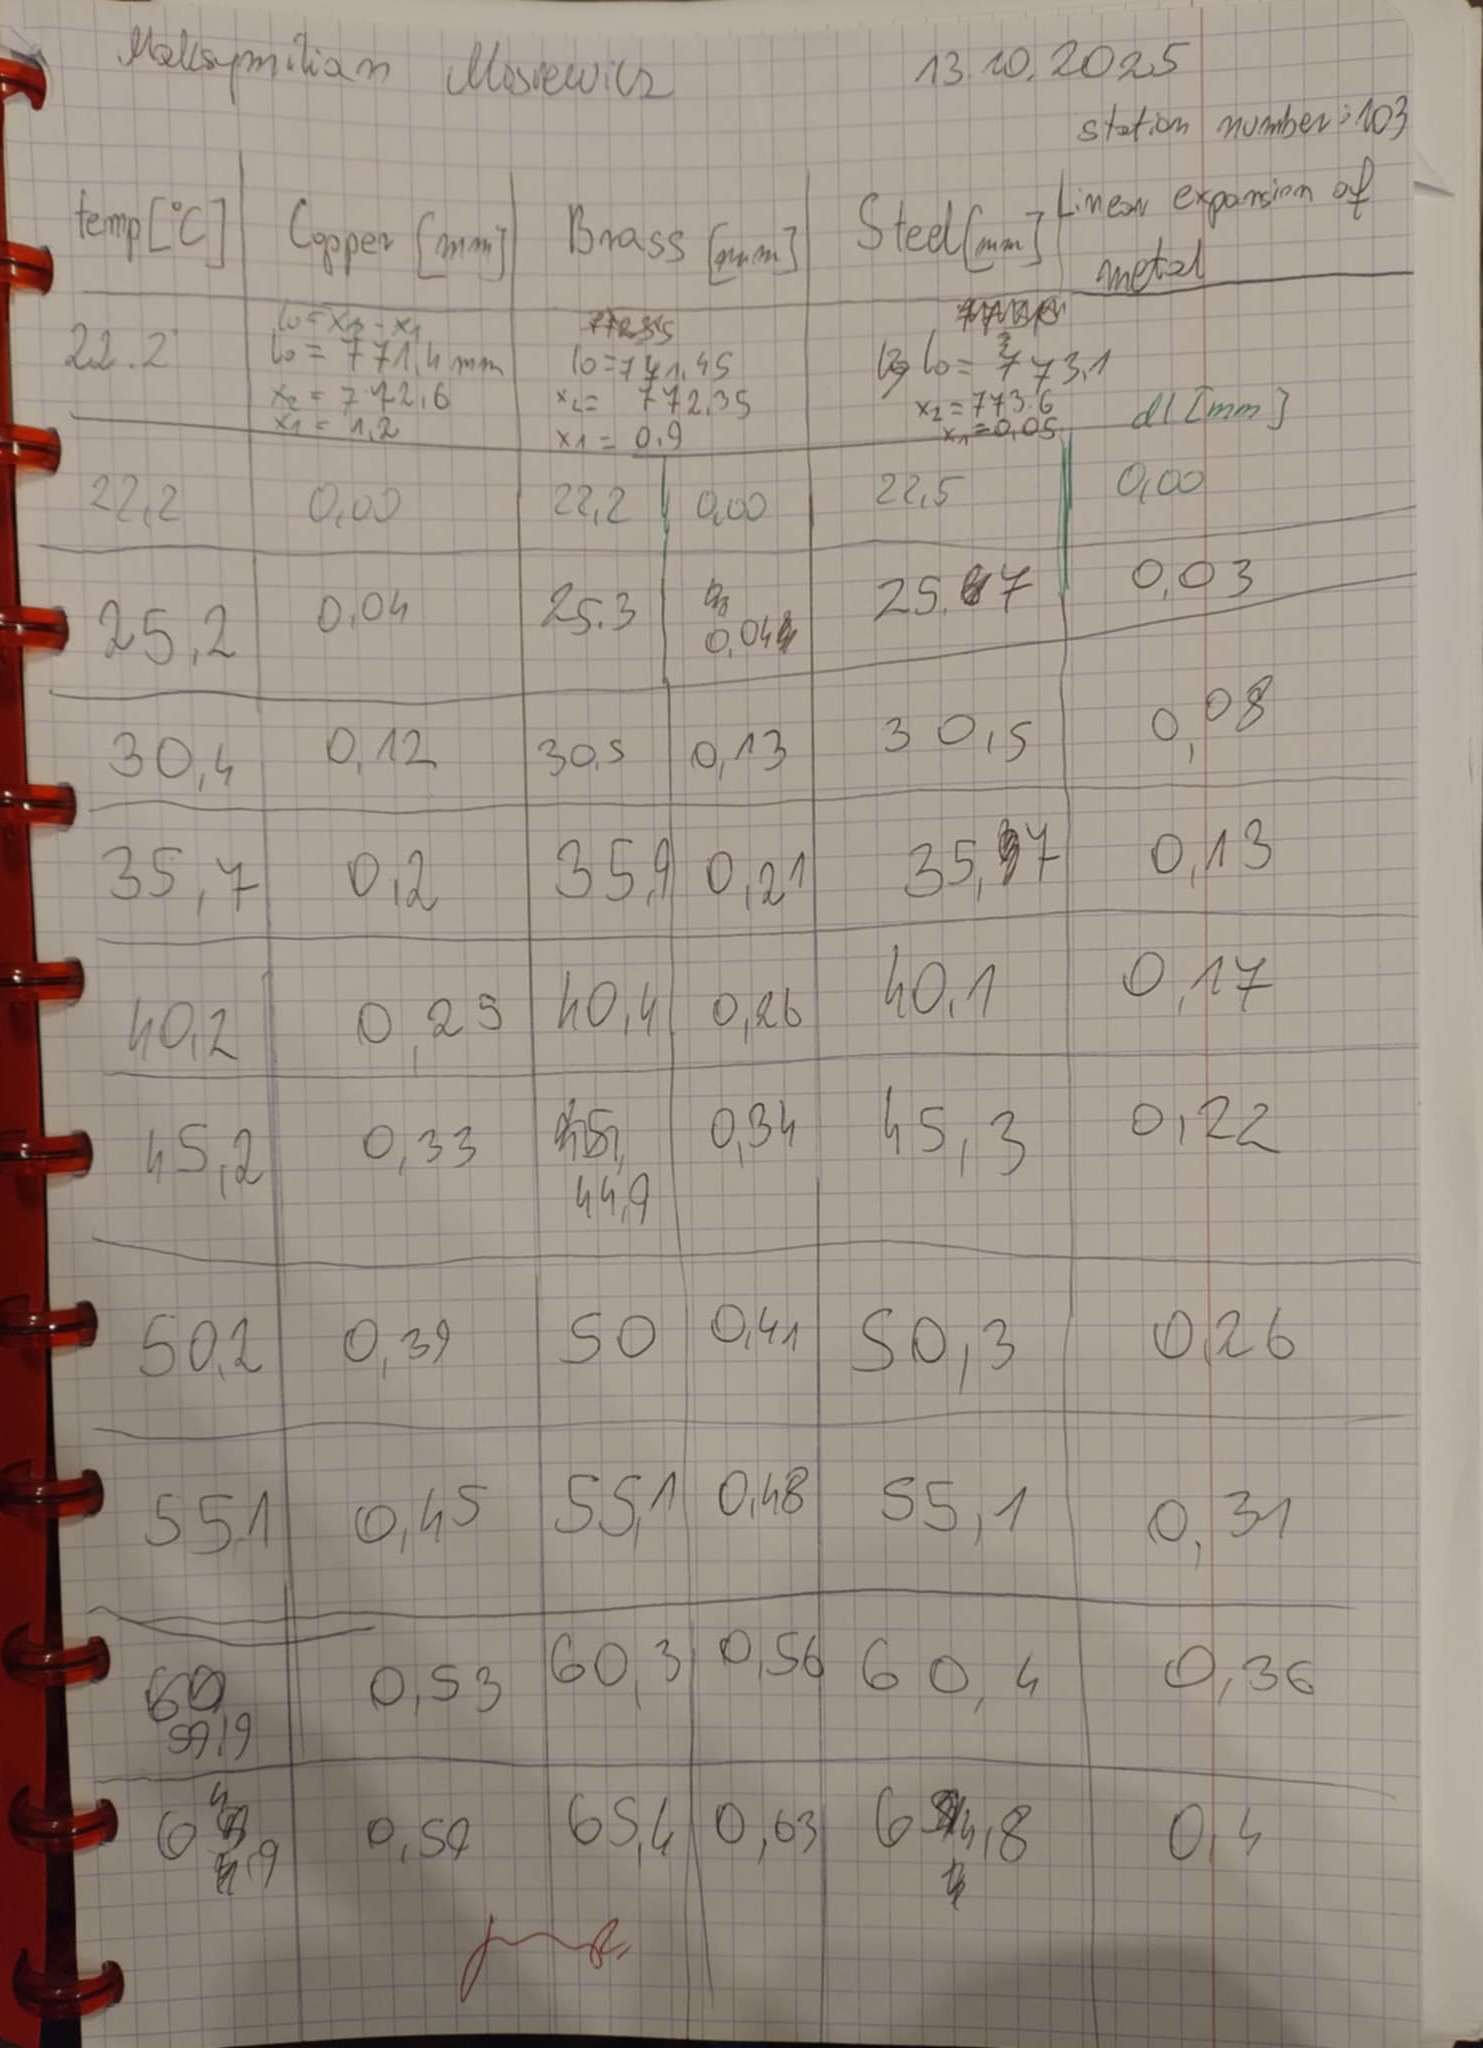
\includegraphics[width=1\textwidth]{figures/measurements.png}
    \caption{Thermal expansion of metal rods.}
    \label{fig:expansion_plot}
\end{figure}

